% Teilauswertung 1

\section{Mittelung und Fouriertransformation}
\label{sec:mittelungAndTrafo}

\paragraph{a)}\textbf{Experimentelle Bestimmung der Fourierentwicklungskoeffizienten}

Im Folgenden wird die Fourierentwicklungskoeffizienten der Sinus, Rechteck und Dreiecksschwingung experimentell bestimmt. Dazu werden die einzelnen Peaks im Fourierspektrum mithilfe von einem Python-Skript (argelextrma Modul aus scipy.signal Paket ermittelt, welche dann den Wert der Fourierentwicklungskoeffizienten für diese Frequenz darstellen. Beachtet werden nur ungerade Vielfache der eingestellten Frequenz. Dies folgt aus Kapitel \ref{sec:fourierseries} bei der nur ungerade Vielfache in der Reihenentwicklung von Rechteck und Dreieckschwingung vorkommen. Die Daten der Amplitude $A$ wurden dabei in dB aufgenommen. Für die Umrechnung der Amplitude in dB zu Volt wird die Gleichung (\ref{eq:spannungpegel}) aus Kapitel \ref{sec:pegel} nach der Spannung $U$ aufgelöst und erhält:
\begin{gather}
    L_U = 20 \log_{10}\left(\frac{U}{U_0}\right)~\Leftrightarrow~U = U_0 \cdot 10^{\frac{L_U}{20}}
    \label{eq:umpegel}
\end{gather}
Zu beachten ist noch, dass die Spannung $U$ die gemessene Effektivspannung ist. Diese Effektivspannung muss mit dem Faktor für die Sinusschwingung aus Kapitel \ref{sec:fourierseries} umgewandelt werden, da die Fourierreihe der jeweiligen Schwingung aus Sinusschwingungen besteht. Die verwendeten Formeln sind dann:
\begin{gather}
    U = U_0 \cdot 10^{\frac{L_U}{20}} \cdot \sqrt{2}  ~\text{mit}~U_0=1\,\text{V}
    \label{eq:umrechnung}
\end{gather}
Die Auswertung ergibt dann Tabelle \ref{tab:fourierkoeff}, in welcher man gut erkennen kann, dass die gemessenen Werte nicht weit von der Theorie abweichen. Dafür wurde die betragsmässige Differenz $\Delta A = \abs{A_{Mess}-A_{Theo}}$ zusätzlich berechnet und graphisch in Abbildung \ref{image:residuum} mit den Fourierspektren der Schwingungen dargestellt. Dabei wurden die theoretischen Werte mit Gleichung (\ref{eq:umpegel}) umgerechnet mit $U = U_{Theo}/\sqrt{2}$. Bei genauerer Betrachtung fällt auf, dass die Kurven für die Rechteckschwingung und der Dreieckschwingung bis zu einer Frequenz $f=9$\,kHz einen ähnlichen Verlauf haben. Danach steigt $\Delta A$ für die Rechteckschwingung stetig bis zu einem Maximum bei 100\,kHz an währenddessen die Dreieckschwingung weiterhin nahe bei 0\,$\mu$V bleibt. Dies kann durch Rauschen in der Messapparatur verursacht worden sein.
\newpage
\begin{center}
    %\textbf{Sinus}\\[0,2cm]
    %\begin{tabular}{l | c | c c c}
    %    $k$ & $f$/kHz &   $A_{Mess}$/V & $A_{Theo}$/V & $\Delta A$/V\\
    %    \hline
    %    1 & 1 &  1,0024 & 1,0000 & 0,0024\\
    %\end{tabular}\\[0,5cm]
    \begin{tabular}{l | c | c c r | c c r}
        \multicolumn{2}{c}{} & \multicolumn{3}{c}{\textbf{Rechteck}} & \multicolumn{3}{c}{\textbf{Dreieck}}\\
        $k$ & $f$/kHz  &   $A_{Mess}$/V & $A_{Theo}$/V & $\Delta A$/$\mu$V  &   $A_{Mess}$/V & $A_{Theo}$/V & $\Delta A$/$\mu$V\\
        \hline
        1  &       1 &  1,276204 &  1,273240 & 2964,00 & 0,812606 &  0,810569 & 2036,48 \\
        2  &       3 &  0,425216 &  0,424413 &  803,00 & 0,090246 &  0,090063 &  183,15 \\
        3  &       5 &  0,254976 &  0,254648 &  328,00 & 0,032489 &  0,032423 &   66,12 \\
        4  &       7 &  0,181976 &  0,181891 &   85,00 & 0,016573 &  0,016542 &   31,10 \\
        5  &       9 &  0,141379 &  0,141471 &   92,00 & 0,009979 &  0,010007 &   27,96 \\
        6  &      11 &  0,115513 &  0,115749 &  236,00 & 0,006700 &  0,006699 &    1,16 \\
        7  &      13 &  0,097574 &  0,097942 &  367,00 & 0,004805 &  0,004796 &    8,75 \\
        8  &      15 &  0,084397 &  0,084883 &  486,00 & 0,003604 &  0,003603 &    1,51 \\
        9  &      17 &  0,074300 &  0,074896 &  596,00 & 0,002806 &  0,002805 &    1,31 \\
        10 &      19 &  0,066309 &  0,067013 &  704,00 & 0,002247 &  0,002245 &    1,82 \\
        11 &      21 &  0,059820 &  0,060630 &  811,00 & 0,001853 &  0,001838 &    1,48 \\
        12 &      23 &  0,054445 &  0,055358 &  913,00 & 0,001530 &  0,001532 &    2,60 \\
        13 &      25 &  0,049915 &  0,050930 & 1014,00 & 0,001298 &  0,001297 &    1,31 \\
        14 &      27 &  0,046045 &  0,047157 & 1112,00 & 0,001116 &  0,001112 &    4,53 \\
        15 &      29 &  0,042696 &  0,043905 & 1209,00 & 0,000963 &  0,000964 &    1,13 \\
        16 &      31 &  0,039764 &  0,041072 & 1308,00 & 0,000846 &  0,000843 &    2,17 \\
        17 &      33 &  0,037185 &  0,038583 & 1398,00 & 0,000737 &  0,000744 &    7,77 \\
        18 &      35 &  0,034885 &  0,036378 & 1493,00 & 0,000654 &  0,000662 &    8,18 \\
        19 &      37 &  0,032824 &  0,034412 & 1588,00 & 0,000591 &  0,000592 &    0,72 \\
        20 &      39 &  0,030967 &  0,032647 & 1680,00 & 0,000521 &  0,000533 &   12,02 \\
        21 &      41 &  0,029284 &  0,031055 & 1771,00 & 0,000480 &  0,000482 &    1,84 \\
        22 &      43 &  0,027747 &  0,029610 & 1863,00 & 0,000433 &  0,000438 &    5,67 \\
        23 &      45 &  0,026338 &  0,028294 & 1956,00 & 0,000395 &  0,000400 &    4,88 \\
        24 &      47 &  0,025044 &  0,027090 & 2046,00 & 0,000362 &  0,000367 &    4,84 \\
        25 &      49 &  0,023854 &  0,025984 & 2130,00 & 0,000335 &  0,000338 &    2,90 \\
        26 &      51 &  0,022747 &  0,024965 & 2218,00 & 0,000312 &  0,000312 &    0,68 \\
        27 &      53 &  0,021718 &  0,024023 & 2305,00 & 0,000280 &  0,000289 &    8,32 \\
        28 &      55 &  0,020760 &  0,023150 & 2390,00 & 0,000264 &  0,000268 &    4,02 \\
        29 &      57 &  0,019863 &  0,022338 & 2475,00 & 0,000255 &  0,000249 &    5,43 \\
        30 &      59 &  0,019024 &  0,021580 & 2557,00 & 0,000237 &  0,000233 &    3,97 \\
        31 &      61 &  0,018230 &  0,020873 & 2642,00 & 0,000218 &  0,000218 &    0,44 \\
        32 &      63 &  0,017489 &  0,020210 & 2721,00 & 0,000205 &  0,000204 &    0,45 \\
        33 &      65 &  0,016786 &  0,019588 & 2802,00 & 0,000194 &  0,000192 &    1,69 \\
        34 &      67 &  0,016126 &  0,019004 & 2878,00 & 0,000181 &  0,000181 &    0,39 \\
        35 &      69 &  0,015501 &  0,018453 & 2951,00 & 0,000170 &  0,000170 &    0,61 \\
    \end{tabular}
    \begin{tabular}{l | c | c c r | c c r}
        \multicolumn{2}{c}{} & \multicolumn{3}{c}{\textbf{Rechteck}} & \multicolumn{3}{c}{\textbf{Dreieck}}\\
        $k$ & $f$/kHz  &   $A_{Mess}$/V & $A_{Theo}$/V & $\Delta A$/$\mu$V  &   $A_{Mess}$/V & $A_{Theo}$/V & $\Delta A$/$\mu$V\\
        \hline  
        36 &      71 &   0,014909 &  0,017933 &  3024,00 & 0,000164 &  0,000161 &   3.33 \\
        37 &      73 &   0,014344 &  0,017442 &  3097,00 & 0,000156 &  0,000152 &   4.20 \\
        38 &      75 &   0,013814 &  0,016977 &  3163,00 & 0,000145 &  0,000144 &   1.37 \\
        39 &      77 &   0,013305 &  0,016536 &  3230,00 & 0,000134 &  0,000137 &   3.04 \\
        40 &      79 &   0,012825 &  0,016117 &  3292,00 & 0,000133 &  0,000130 &   3.28 \\
        41 &      81 &   0,012368 &  0,015719 &  3351,00 & 0,000129 &  0,000124 &   5.11 \\
        42 &      83 &   0,011932 &  0,015340 &  3408,00 & 0,000122 &  0,000118 &   4.17 \\
        43 &      85 &   0,011522 &  0,014979 &  3457,00 & 0,000116 &  0,000112 &   4.29 \\
        44 &      87 &   0,011128 &  0,014635 &  3506,00 & 0,000111 &  0,000107 &   4.24 \\
        45 &      89 &   0,010757 &  0,014306 &  3549,00 & 0,000100 &  0,000102 &   2.13 \\
        46 &      91 &   0,010407 &  0,013992 &  3585,00 & 0,000106 &  0,000098 &   8.08 \\
        47 &      93 &   0,010077 &  0,013691 &  3614,00 & 0,000098 &  0,000094 &   4.35 \\
        48 &      95 &   0,009761 &  0,013403 &  3641,00 & 0,000090 &  0,000090 &   0.64 \\
        49 &      97 &   0,009467 &  0,013126 &  3659,00 & 0,000089 &  0,000086 &   2.70 \\
        50 &      99 &   0,009193 &  0,012861 &  3668,00 & 0,000088 &  0,000083 &   5.51 \\
        51 &     101 &   0,008936 &  0,012606 &  3671,00 & 0,000087 &  0,000079 &   7.23 \\
        52 &     103 &   0,008699 &  0,012362 &  3662,00 & 0,000089 &  0,000076 &  13,00 \\
        53 &     105 &   0,008479 &  0,012126 &  3647,00 & 0,000079 &  0,000074 &   5.97 \\
        54 &     107 &   0,008283 &  0,011899 &  3617,00 & 0,000084 &  0,000071 &  13,70 \\
        55 &     109 &   0,008101 &  0,011681 &  3580,00 & 0,000081 &  0,000068 &  13,08 \\
        56 &     111 &   0,007937 &  0,011471 &  3534,00 & 0,000080 &  0,000066 &  13,76 \\
        57 &     113 &   0,007803 &  0,011268 &  3465,00 & 0,000077 &  0,000063 &  13,08 \\
        58 &     115 &   0,007687 &  0,011072 &  3385,00 & 0,000076 &  0,000061 &  15,02 \\
        59 &     117 &   0,007586 &  0,010882 &  3297,00 & 0,000080 &  0,000059 &  20,31 \\
        60 &     119 &   0,007514 &  0,010699 &  3186,00 & 0,000076 &  0,000057 &  18,57 \\
        61 &     121 &   0,007456 &  0,010523 &  3066,00 & 0,000075 &  0,000055 &  19,14 \\
        62 &     123 &   0,007423 &  0,010352 &  2929,00 & 0,000078 &  0,000054 &  24,34 \\
    \end{tabular}  
    \captionof{table}{Vergleich Fourierentwicklungskoeffizienten in Theorie und Praxis}
    \label{tab:fourierkoeff}
\end{center}
\begin{center}
    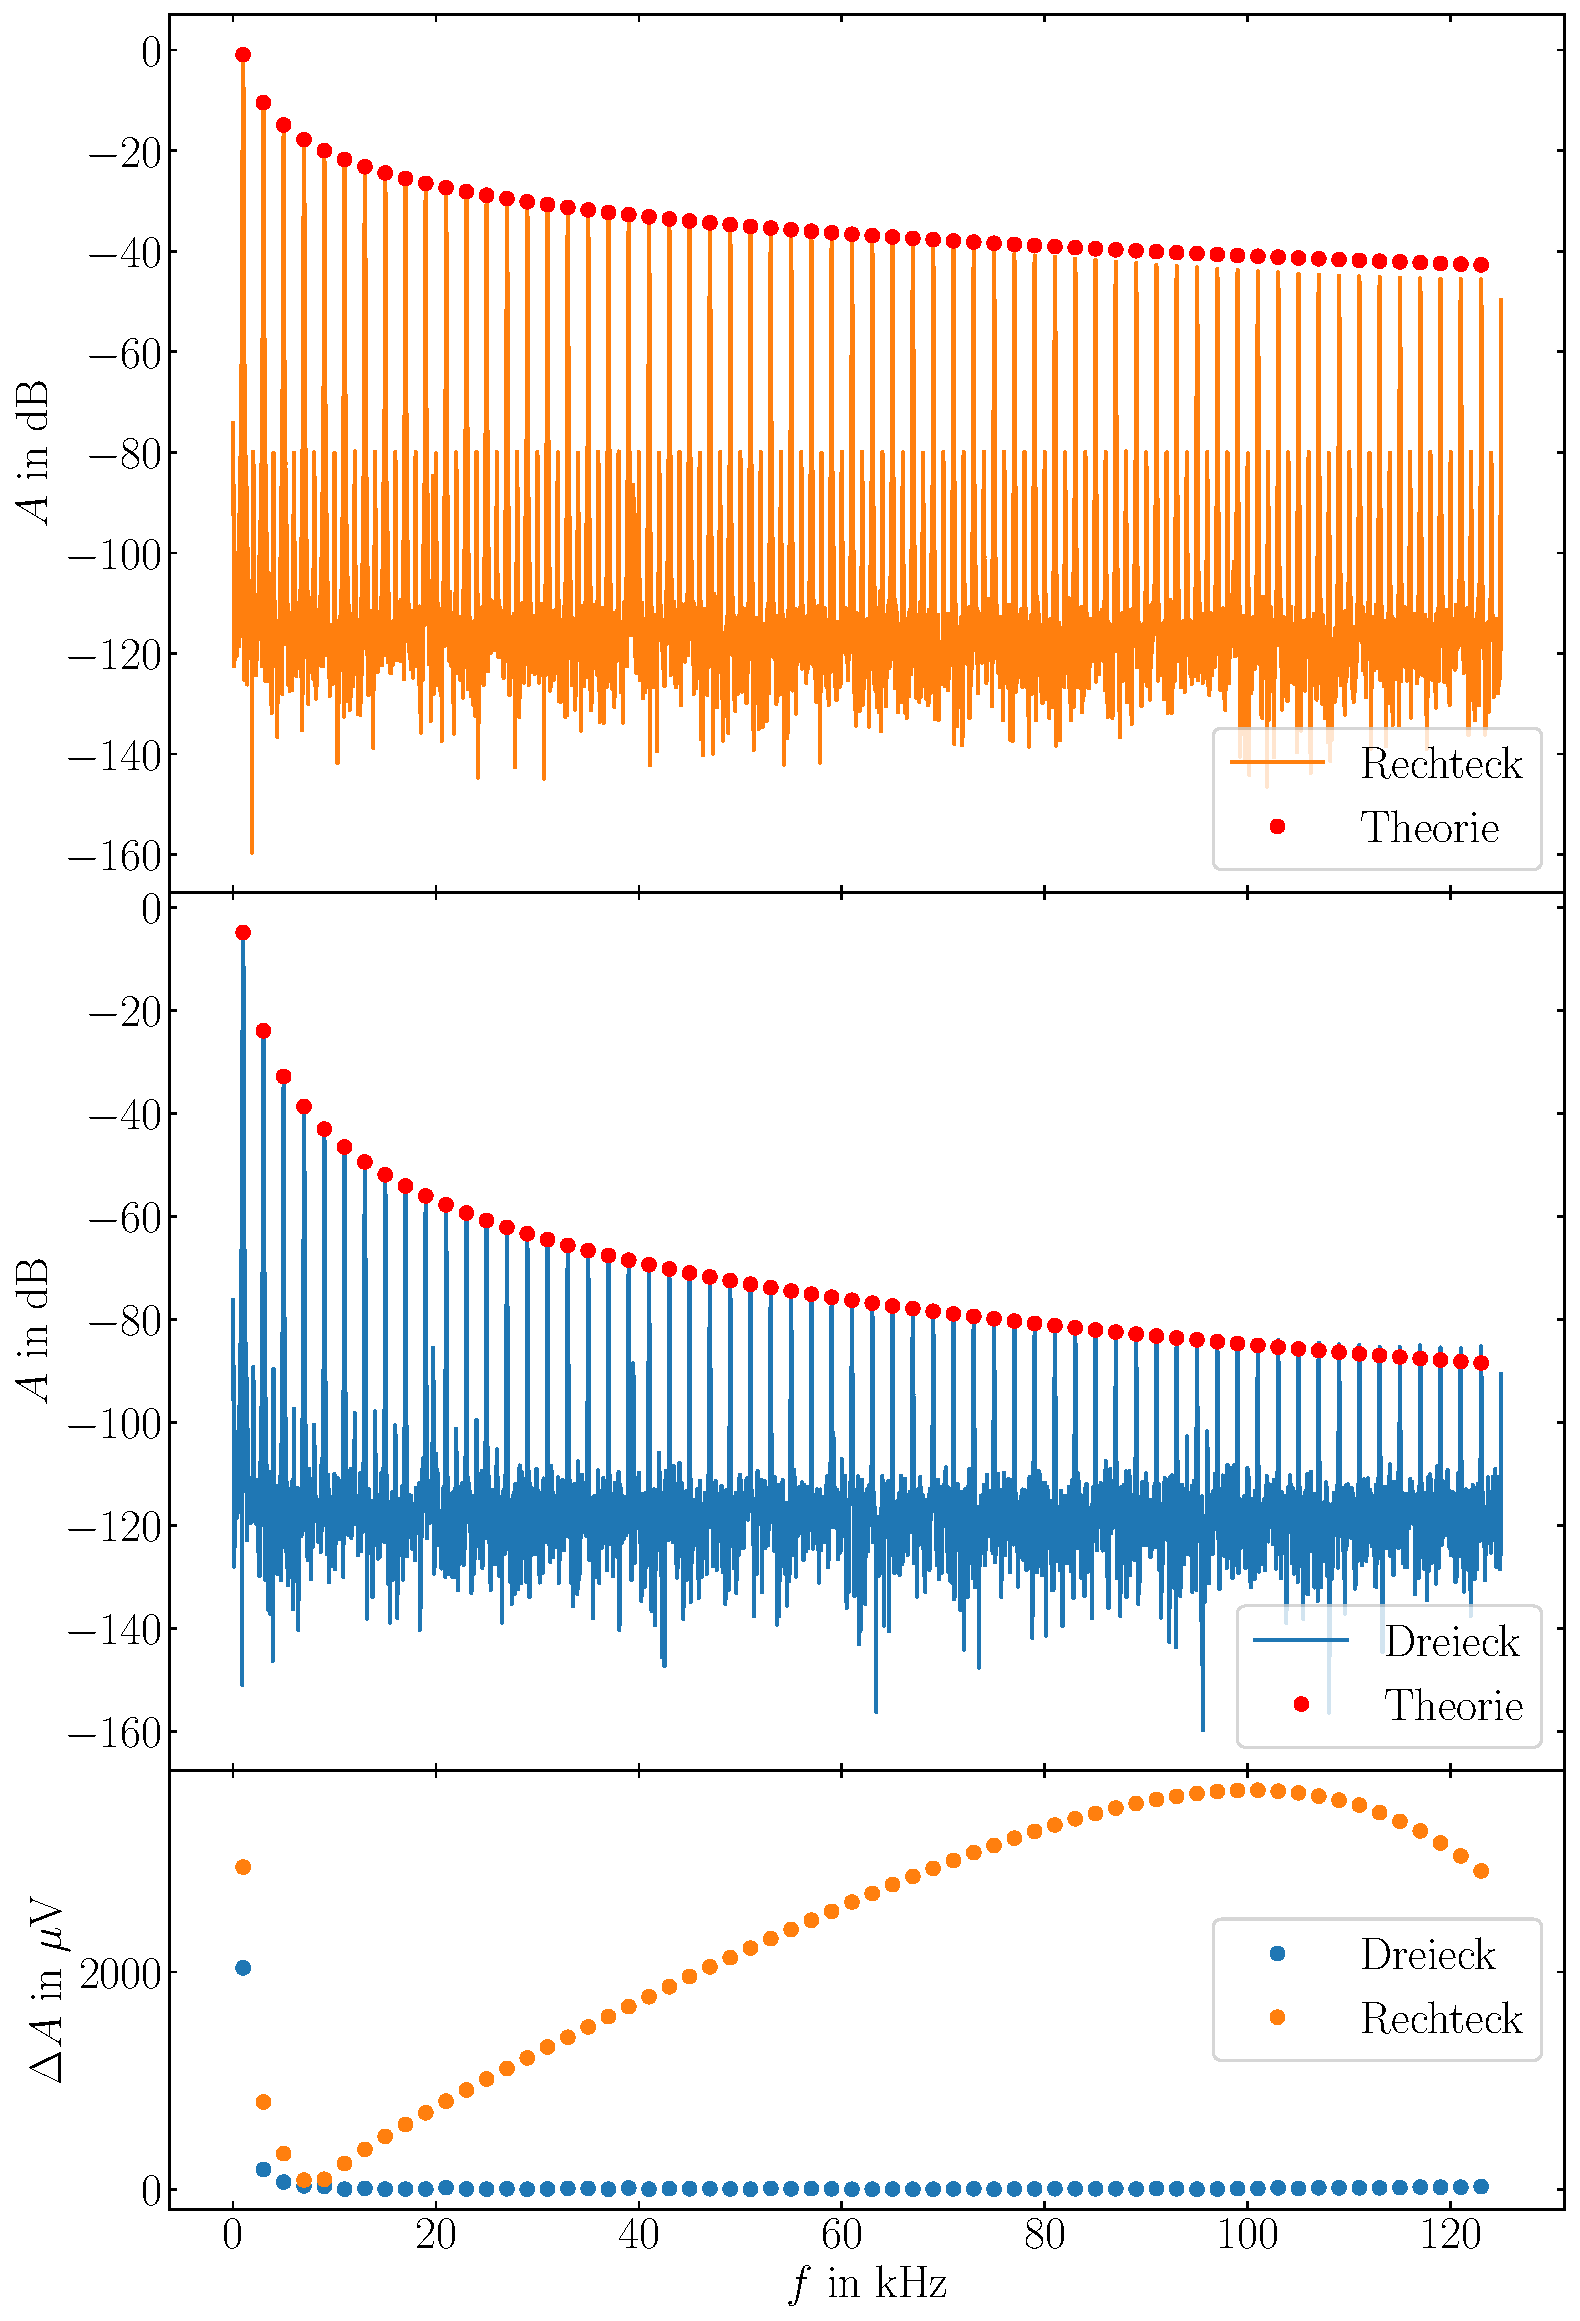
\includegraphics[scale = 0.5]{Manuel/41/Residuum.pdf}
    \captionof{figure}{Betragsmässige Differenz der Messwerte und Theorie mit den jeweiligen Fourierspektrum der Schwingungsform mit Theorie}
    \label{image:residuum}
\end{center}


\newpage
\paragraph{b)}\textbf{Fourierspektrum Sinusschwingung}

Dieser Teil behandelt das Fourierspektrum der Sinusschwingung bei 1\,V Amplitude.
\begin{center}
    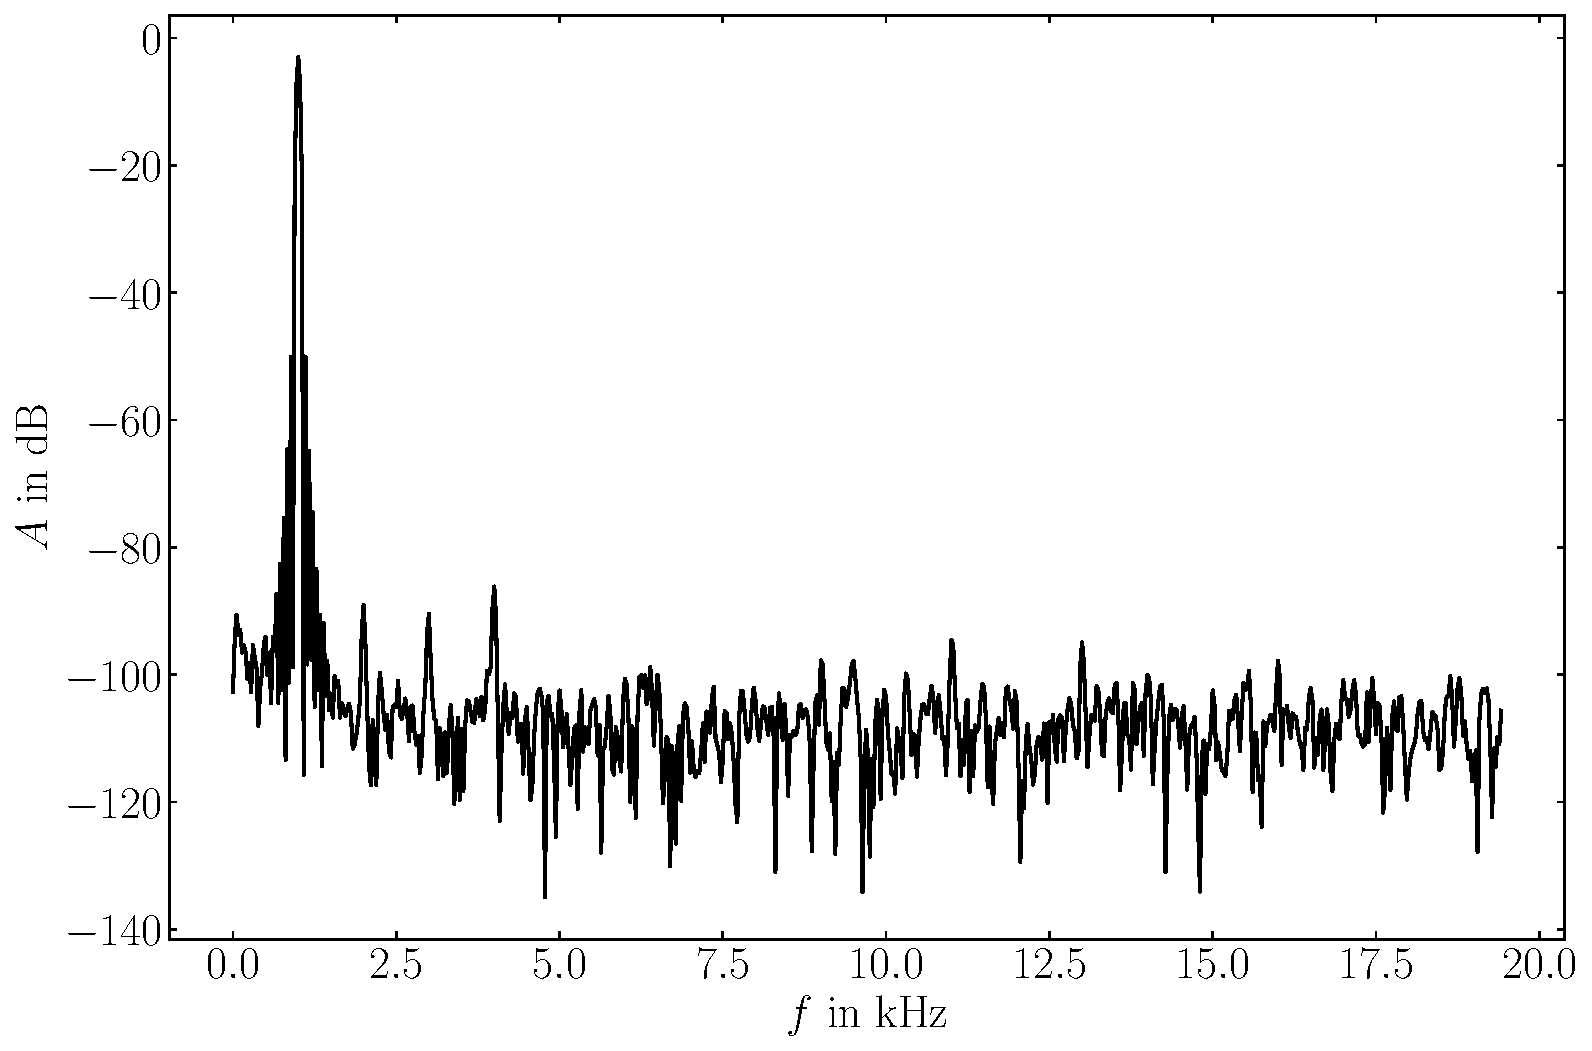
\includegraphics[scale = 0.5]{Manuel/41/FourierSinus.pdf}
    \captionof{figure}{Fourierspektrum der Sinusschwingung}
    \label{image:fourierSinus}
\end{center}
Wie in Abbildung \ref{image:fourierSinus} zu sehen, ist ein deutlich ausgeprägter Peak bei einer Frequenz von 1\,kHz zu erkennen. Nach Kapitel \ref{sec:fourierseries} sollte aber das Fourierspektrum nur einen Peak in Form einer Delta-Funktion bei der eingestellten Frequenz besitzen. Dies ist in der realen Welt aufgrund von Rauschen nicht möglich, wodurch der Hauptpeak bei 1\,kHz als eine breite Delta-Funktion gemessen wird. Weiterhin ist in Abbildung \ref{image:fourierSinus} neben dem Hauptpeak deutlich noch weiter kleinere Peaks zu erkennen, welche selbst in einem Abstand von 1\,kHz auftreten. Diese Peaks werden durch die Umgebungseinflüsse aus Kapitel \ref{sec:umwelt} und durch die Netzspannungsquelle selbst verursacht.


\newpage
\paragraph{c)}\textbf{Einfluss Mittelung auf Rechteckschwingung}

Nun wird der Einfluss der Anzahl der Mittelung $N$ auf eine Rechteckschwingung mit einer Amplitude $U_0=$ 1\,V mit einem Rauschen der Bandbreite $f_{Band}=$ 20\,MHz und einer AM Depth $=$ 120\,\% betrachtet.
In Abbildung \ref{image:einflussMittelung} ist zu erkennen, dass sich mit der Zunahme der Anzahl der Mittelungen $N$ der Signal/Rausch-Abstand $d$ zunimmt. Dies war zu erwarten, da schon wie in Kapitel \ref{sub:mittelung} erklärt, bei der Mittelung das Signal des Rauschens nur um den Faktor $\sqrt{N}$ zunimmt, während das Signal der Rechteckschwingung proportional zur Wiederholung anwächst. Um diesen Umstand graphisch darzustellen werden zuerst die Peaks der Rechteckschwingung und der Median bei jeder Mittelung mit einem Python-Skript bestimmt. Der Median jeder Mittelung ist in Abbildung \ref{image:mittelung} als \textit{gestrichelte Linie} in zugehöriger Farbe mit eingezeichnet. Der Signal/Rausch-Abstand $d$ wird dann mit der folgenden Formel bestimmt:
\begin{gather}
    d = \abs{\text{Median} - \text{Maxima}}
\end{gather}
Als Maxima wird der Wert des ersten Peaks verwendet, welcher -6.91\,dB beträgt. Die Berechnung ergibt dann folgende Tabelle:
\begin{center}
    \begin{tabular}{l | c}
        $N$ & $d$/dB\\
        \hline
        0   & 60,28 \\
        10  & 70,61 \\
        50  & 77,65 \\
        100 & 80,39 \\
    \end{tabular}
\end{center}
Da die Werte in dB angegeben sind, muss die Fit-Funktion logaritmisch sein. Der Fit wird mit dem Modul curve\_fit aus dem scipy.optimize Paket erstellt. Die Funktion hat dabei die Form:
\begin{gather}
    \begin{aligned}
       %&d(N) = a\cdot\sqrt{N} + t &\xrightarrow{\text{Fit}} &~~d(N) = 1.99\,\text{dB}\cdot\sqrt{N} + 62.17\,\text{dB} \\
       &d(N) = a\cdot\ln(\sqrt{N+1}) + t &\xrightarrow{\text{Fit}} &~~d(N) = 8,77\,\text{dB}\cdot\ln(\sqrt{N+1}) + 60.24\,\text{dB} \\
    \end{aligned}
\end{gather}
In Abbildung \ref{image:abstandMittelung} erkennt man deutlich, dass der Fit mit der Theorie gut übereinstimmt, was diese wiederum bestätigt. Womit sich sagen lässt, dass sich der Signal/Rausch-Abstand $d$ mit zunehmender Mittelung $N$ vergrößert und es somit möglich ist, das Signal besser aufzulösen.
%In Abbildung \ref{image:abstandMittelung} erkennt man deutlich, dass die natürliche Logarithmus-Funktion besser den Verlauf der Datenpunkten entspricht als die theoretisch erwartete Wurzel-Funktion. Dies kann mit der Wahl der Berechnung des Signal/Rausch-Abstands zusammenhängen. Dennoch lässt sich sagen, dass sich der Signal/Rausch-Abstand $d$ mit zunehmender Mittelung $N$ vergrößert und es somit möglich ist, das Signal besser aufzulösen.
\newpage
\begin{center}
    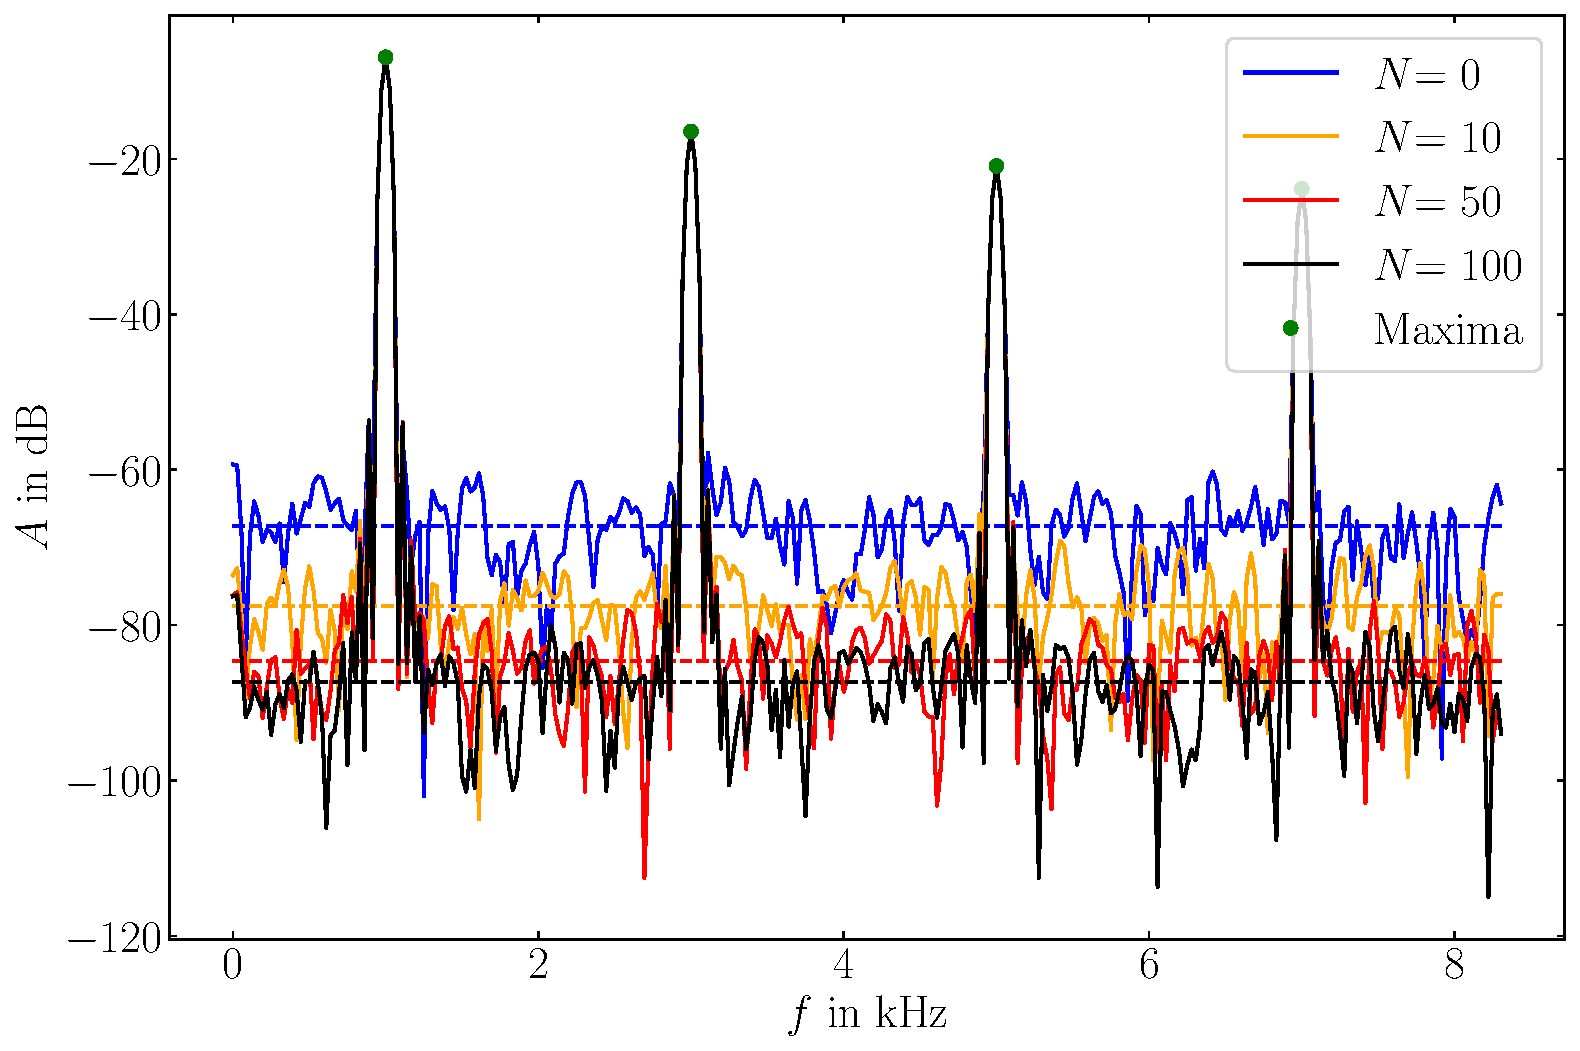
\includegraphics[scale = 0.5]{Manuel/41/Mittelung.pdf}
    \captionof{figure}{Einfluss der Mittelung auf Fourierspektrum einer Rechteckschwingung}
    \label{image:einflussMittelung}
\end{center}
\begin{center}
    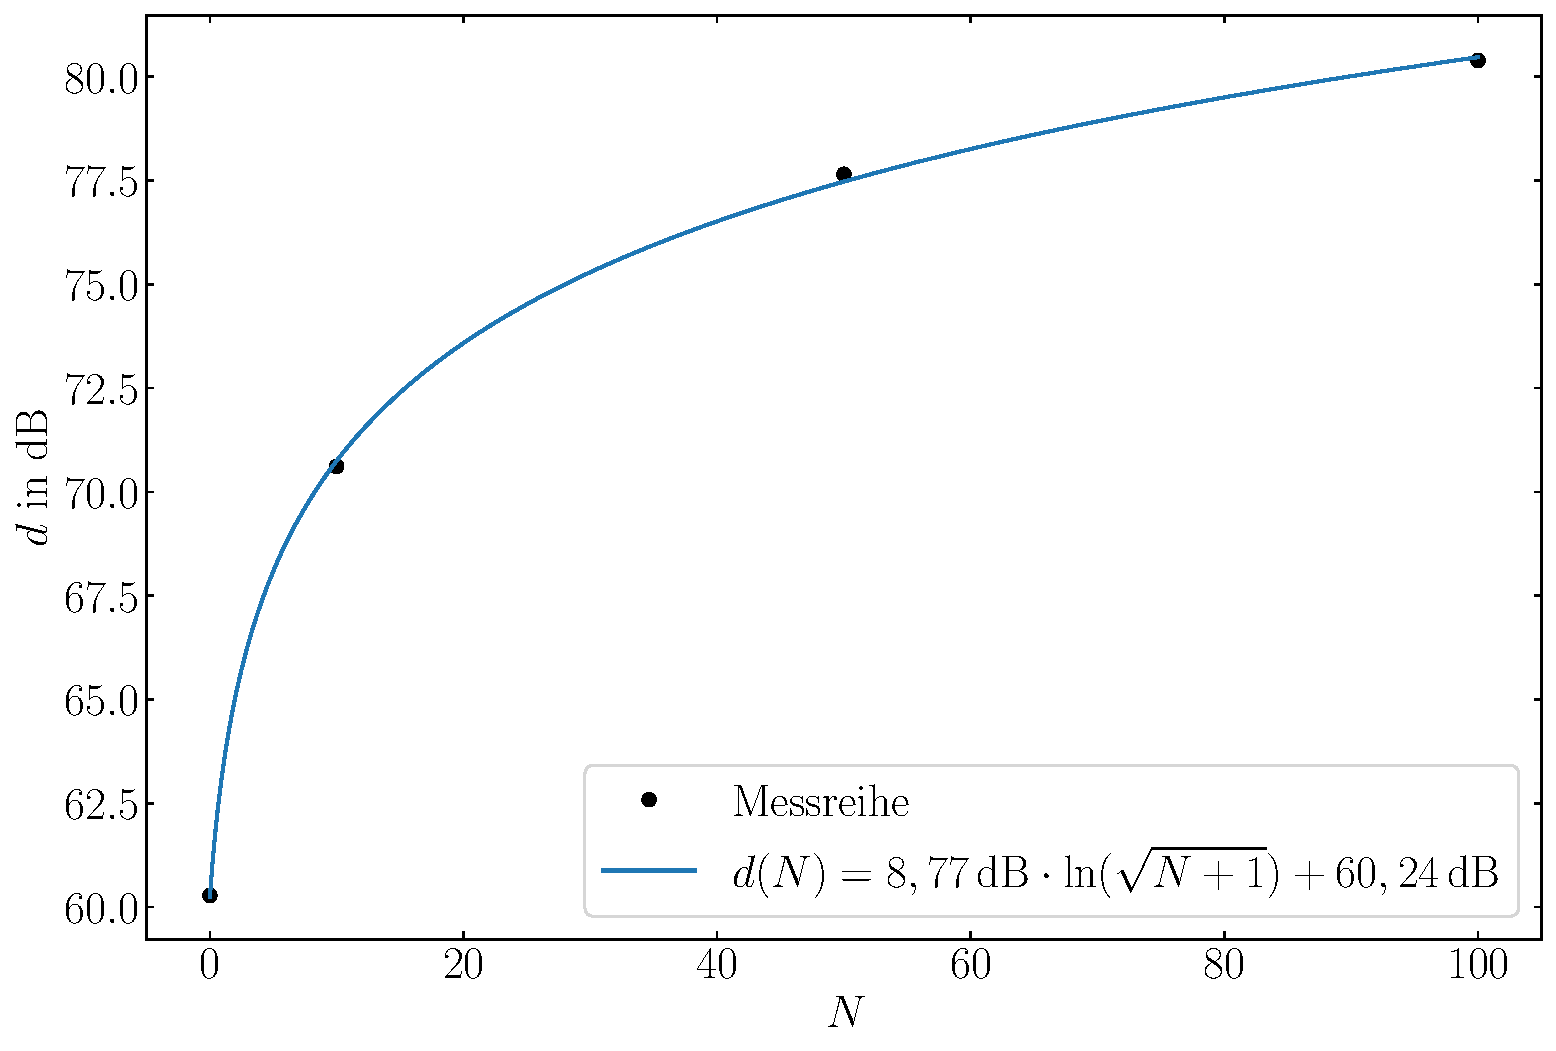
\includegraphics[scale = 0.5]{Manuel/41/MittlungAbstand.pdf}
    \captionof{figure}{Signal-Rausch Abstand in Abhängigkeit der Mittelungen $N$}
    \label{image:abstandMittelung}
\end{center}

\newpage
\paragraph{d)}\textbf{Einfluss Signal/Rausch-Abstand auf zeitliche Signalform}

Als weiteres wird der Einfluss des Signal/Rausch-Verhältnis $V_{SR}$ auf die Signalform einer Rechteckschwingung mit einer Amplitude $U_0=$ 1\,V und einen Bandbreite\\$f_{Band}=$ 20\,MHz betrachtet.
In Abbildung \ref{image:sigRauRechtAll} ist zuerst der Einfluss des Signal/Rausch-Abstands auf die komplette Rechteckschwingung dargestellt. Schon hier erkennt man, dass mit höherem Signal/Rausch-Verhältnis das \enquote{Ausschlagen} der Amplitude des Rauschens zunimmt. Noch deutlich ist dies im Ausschnitt des oberen Umkehrpunkts der Rechteckschwingung in Abbildung \ref{image:sigRauRechtAll} zu erkennen. Dies bedeutet, dass für kleine $V_{SR}$ das Verhältnis aus Nutzsignal und Störsignal (Rauschen) abnimmt, aber der Signal/Rausch-Abstand $d$ zunimmt und somit das Rauschen weniger Anteil am eigentlichen Signal hat. Die Änderung des Signal/Rausch-Verhältnis $V_{SR}$ hat aber keinen generellen Einfluss auf den Verlauf der Signalform der Rechteckschwingung. 
\begin{center}
    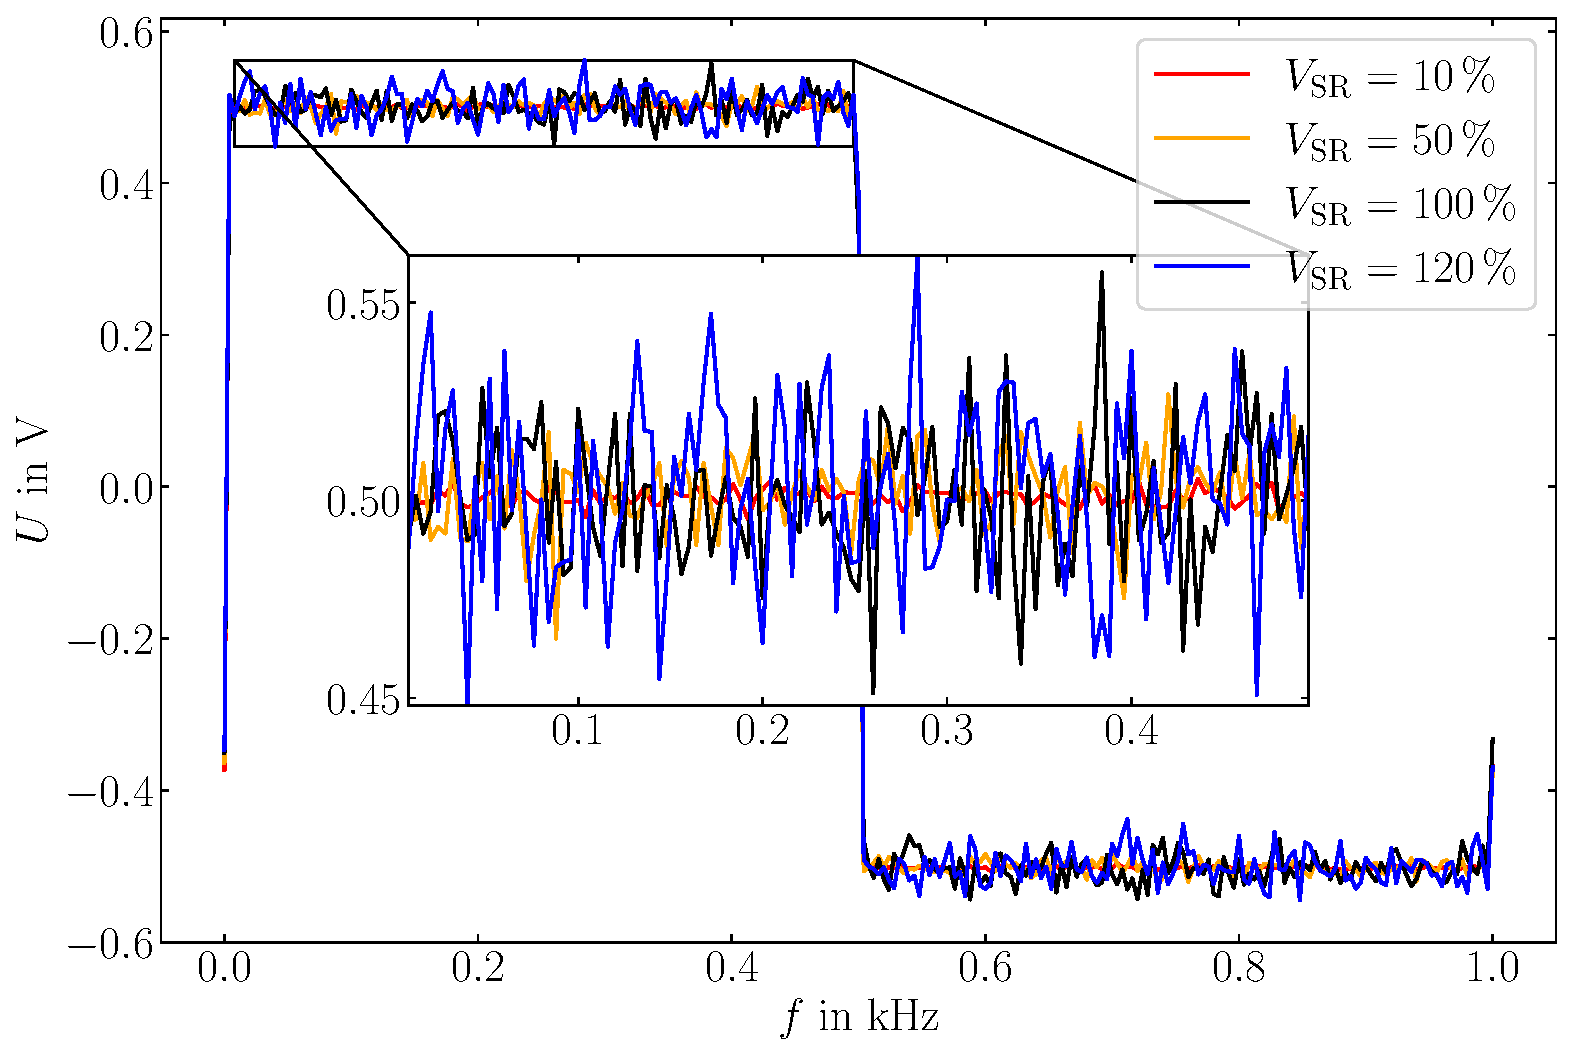
\includegraphics[scale = 0.5]{Manuel/41/SignalRauschAbstandAll.pdf}
    \captionof{figure}{Einfluss Signal/Rausch-Abstand mit Ausschnitt vom obere Umkehrpunkt der Rechteckschwingung}
    \label{image:sigRauRechtAll}
\end{center}
\newpage
%\begin{center}
%    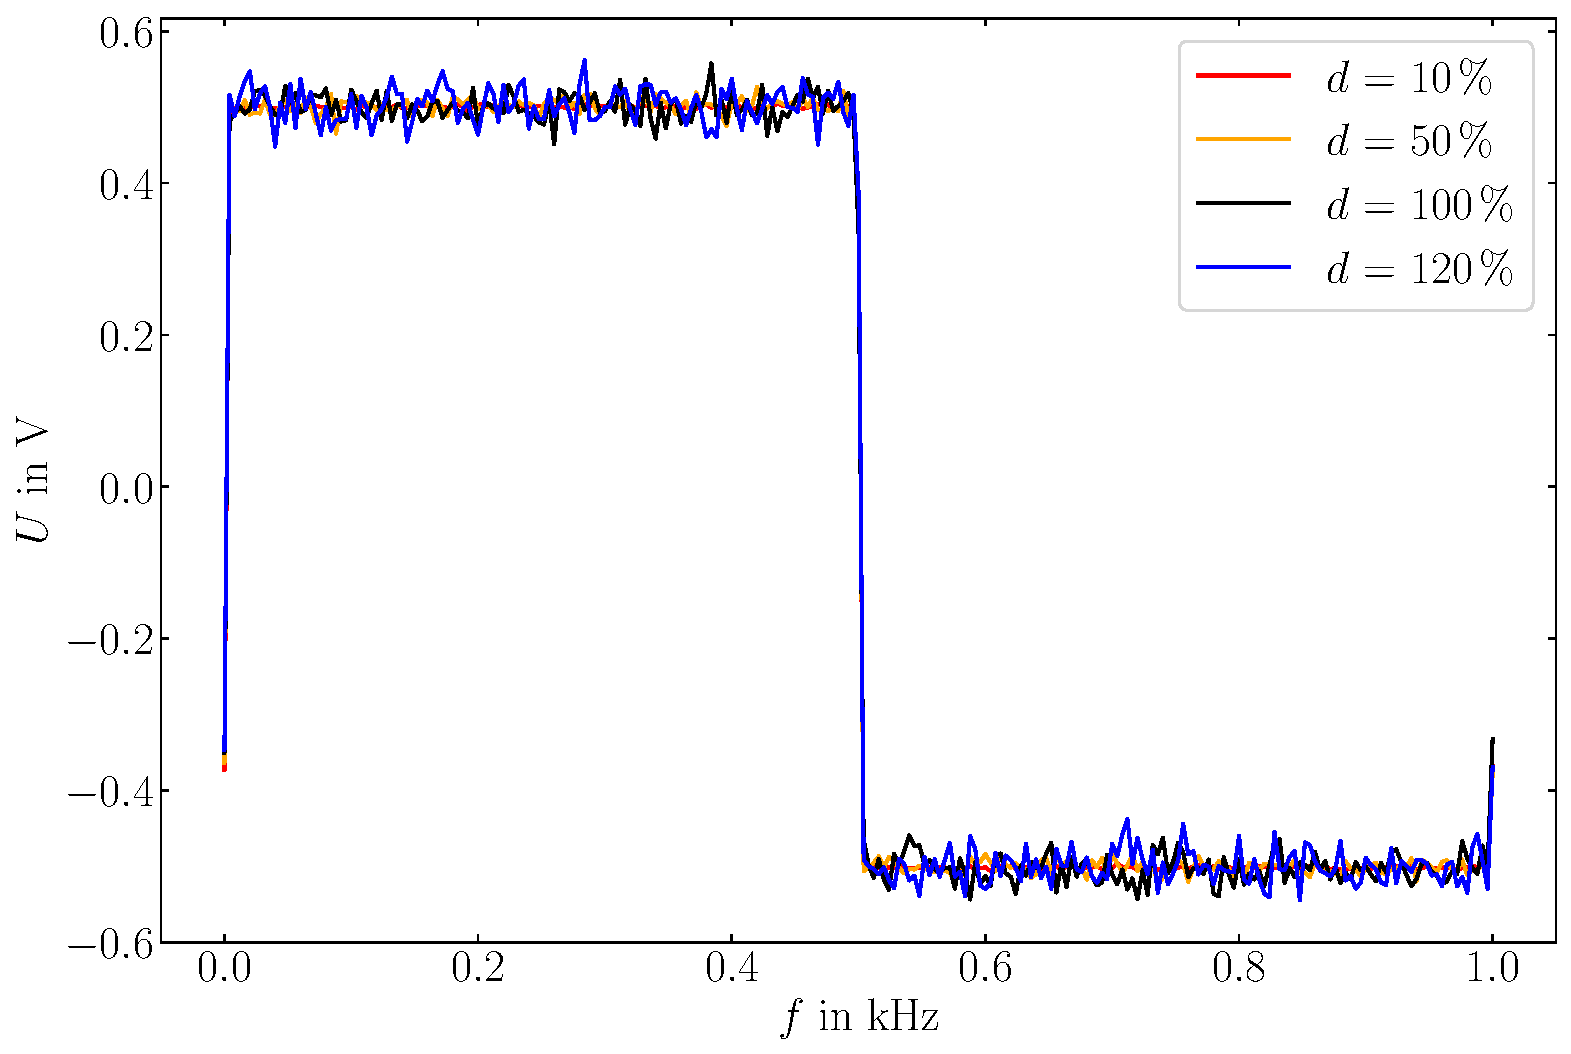
\includegraphics[scale = 0.5]{Manuel/41/SignalRauschAbstandKomplett.pdf}
%    \captionof{figure}{Einfluss Signal/Rausch-Abstand auf komplette Rechteckschwingung}
%    \label{image:sigRauRechtKomplett}
%\end{center}
%\begin{center}
%    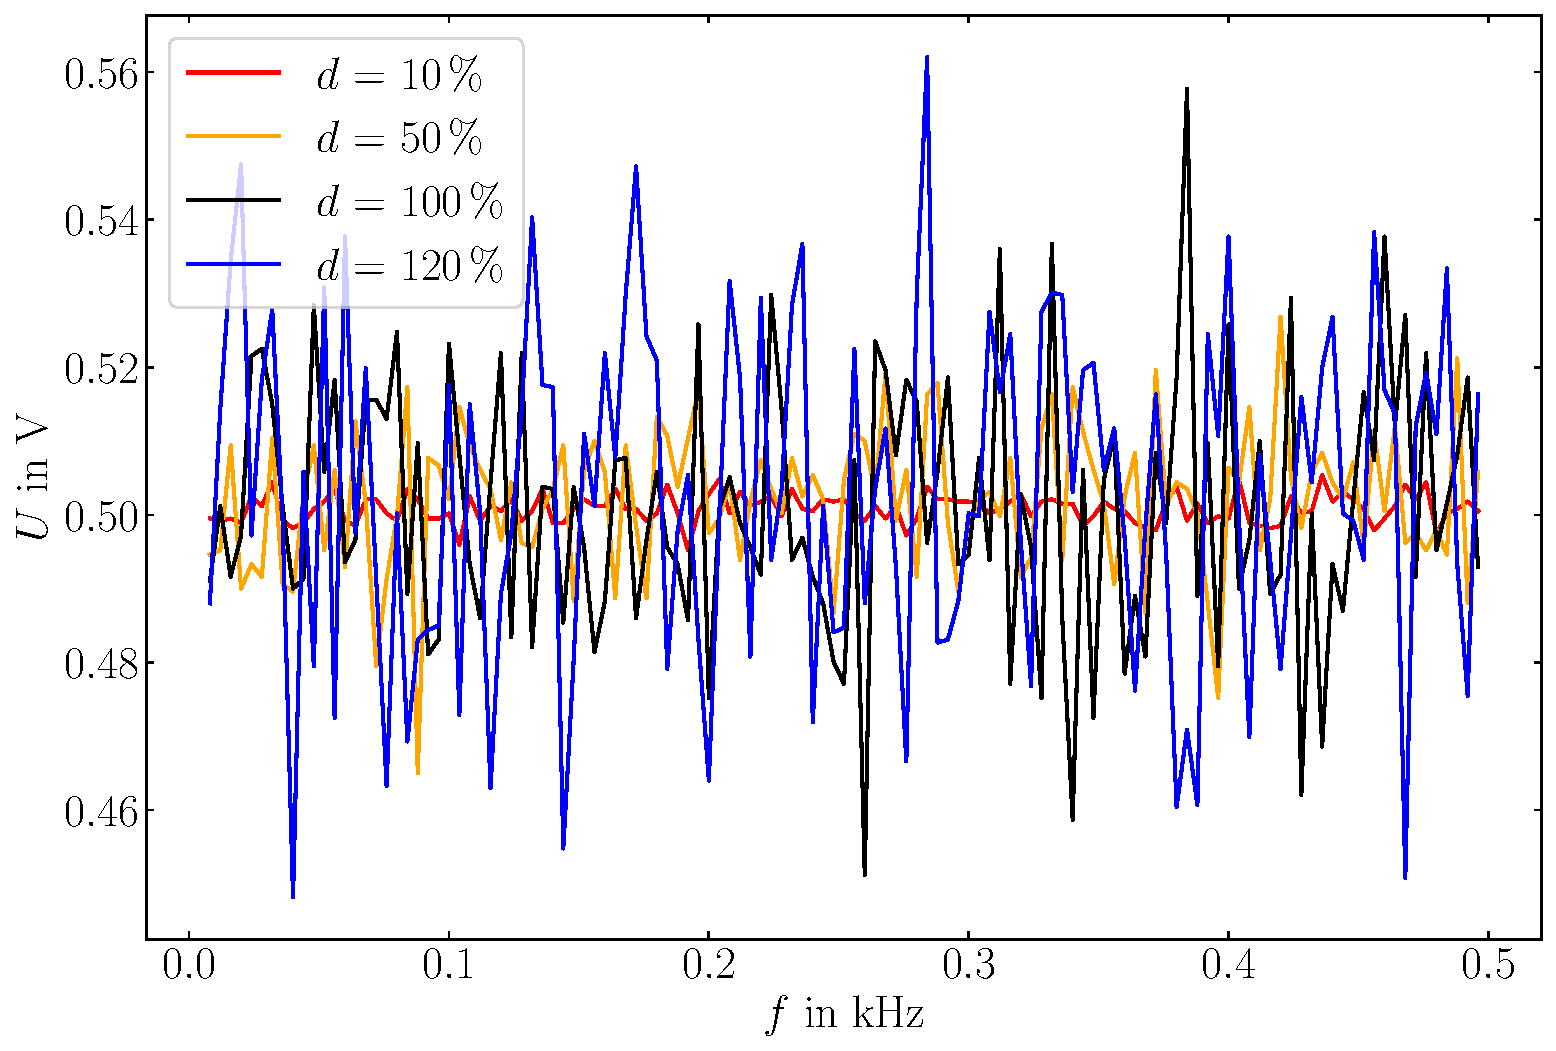
\includegraphics[scale = 0.5]{Manuel/41/SignalRauschAbstand.pdf}
%    \captionof{figure}{Einfluss Signal/Rausch-Abstand im Ausschnitt vom obere Umkehrpunkt der Rechteckschwingung}
%    \label{image:sigRauRecht}
%\end{center}


\paragraph{e)}\textbf{Einfluss Bandbreite auf zeitliche Signalform}

Zuletzt in diesem Kapitel wird der Einfluss der Bandbreite auf die zeitliche Signalform besprochen. Dabei wird wieder eine Rechteckschwingung mit einer Amplitude\\ $U_0=$ 1\,V und einem Signal/Rausch-Abstand $d=$ 100\,\% verwendet. In Abbildung \ref{image:bandbreiteRechtKomplett} wird erneut eine komplette Rechteckschwingung gezeigt. Darauf erkennt man, dass der Funktionsgenerator die Form des Rechtecksignals mit kleineren Bandbreiten $f_{Band}$ nicht mehr erzeugen kann. Vor allem bei Frequenzen unter 100\,kHz. Aber auch eine Zunahme des Rauschens ist zu erkennen, wenn die Bandbreite kontinuierlich abnimmt. Dies bestätigt auch das Fourierspektrum (Abb. \ref{image:bandbreiteRechtFourier}). Darin ist eine Zunahme des Signal/Rausch-Abstands $d$ zu erkennen, was bedeutet, dass bei höheren Bandbreiten das Rauschen auf dem Rechtecksignal abnimmt. In Abbildung \ref{image:bandbreiteRecht} kann man dies noch genauer betrachten.
\begin{center}
    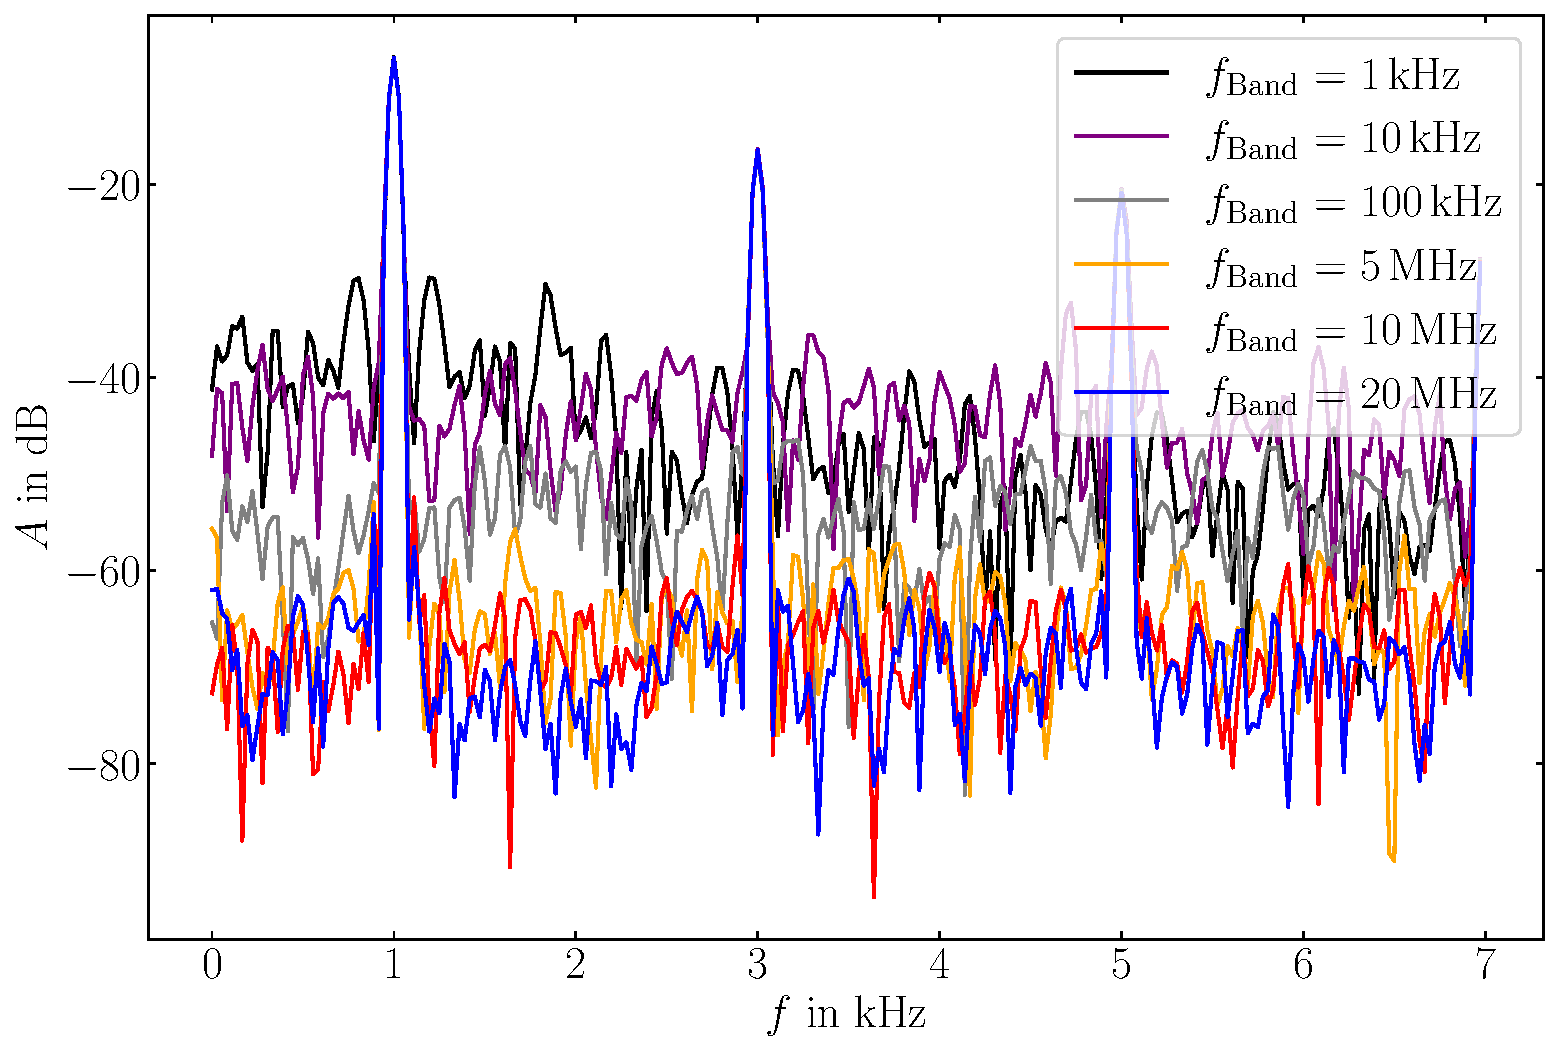
\includegraphics[scale = 0.5]{Manuel/41/BandbreiteFourier.pdf}
    \captionof{figure}{Einfluss Bandbreite auf Rechteckschwingung im Fourierspektrum}
    \label{image:bandbreiteRechtFourier}
\end{center} 
\newpage
\begin{center}
    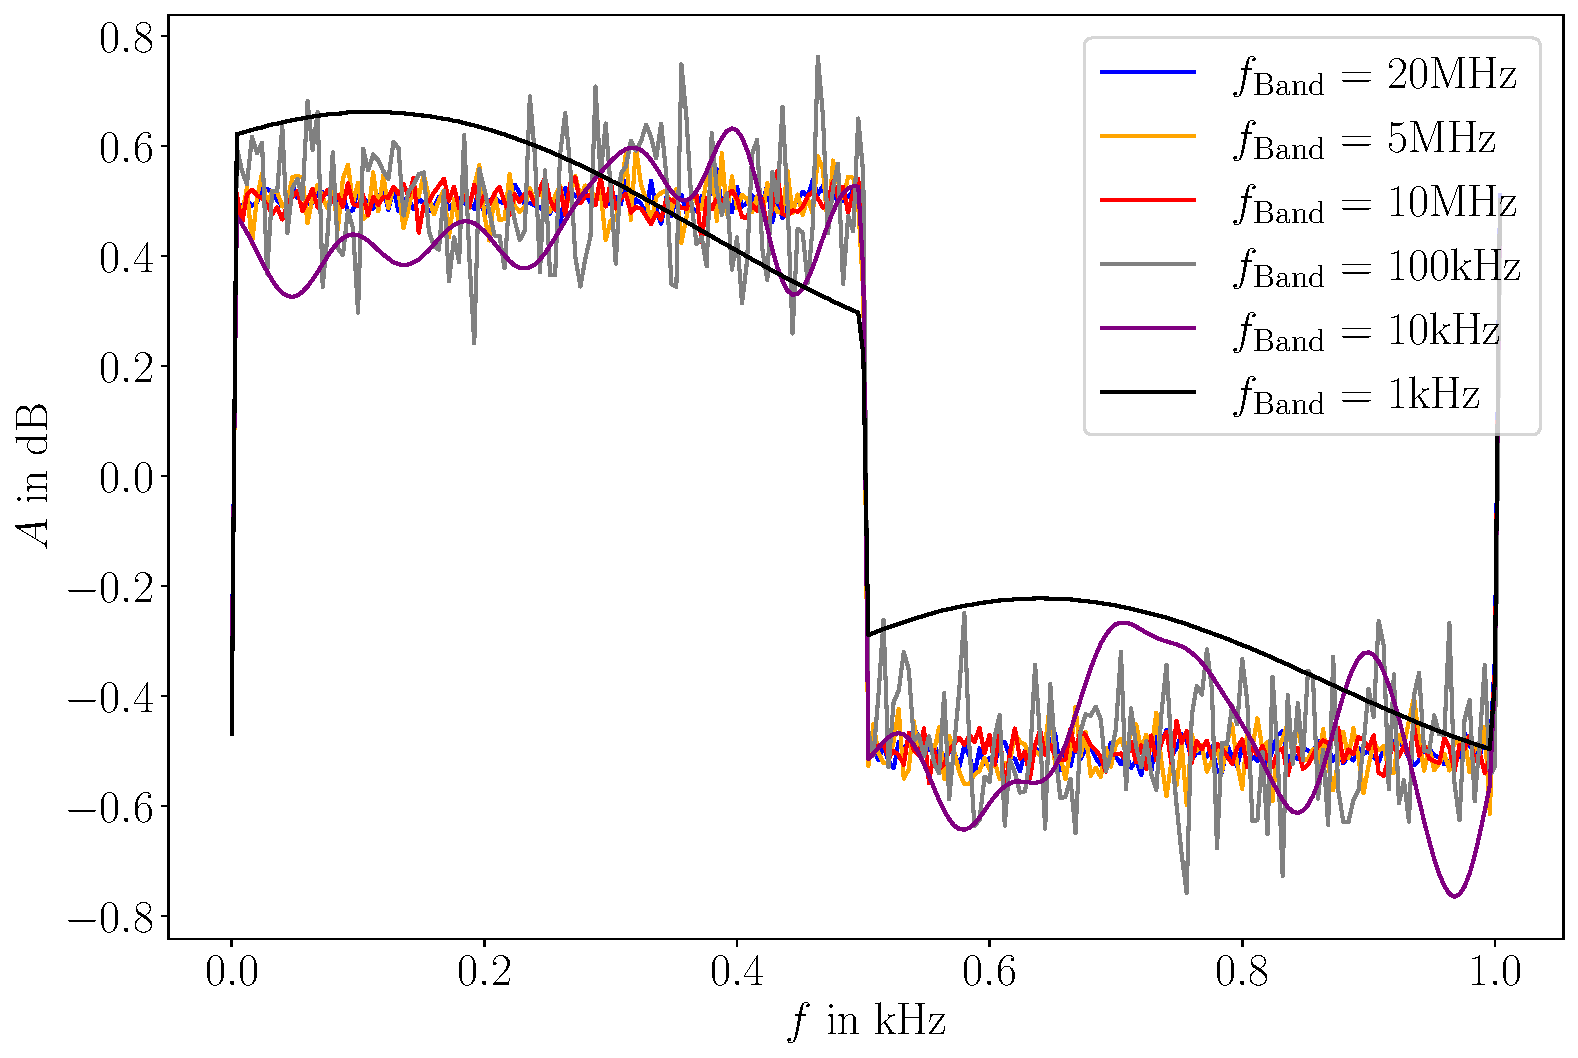
\includegraphics[scale = 0.5]{Manuel/41/BandbreiteKomplett.pdf}
    \captionof{figure}{Einfluss Bandbreite auf komplette Rechteckschwingung}
    \label{image:bandbreiteRechtKomplett}
\end{center}
\begin{center}
    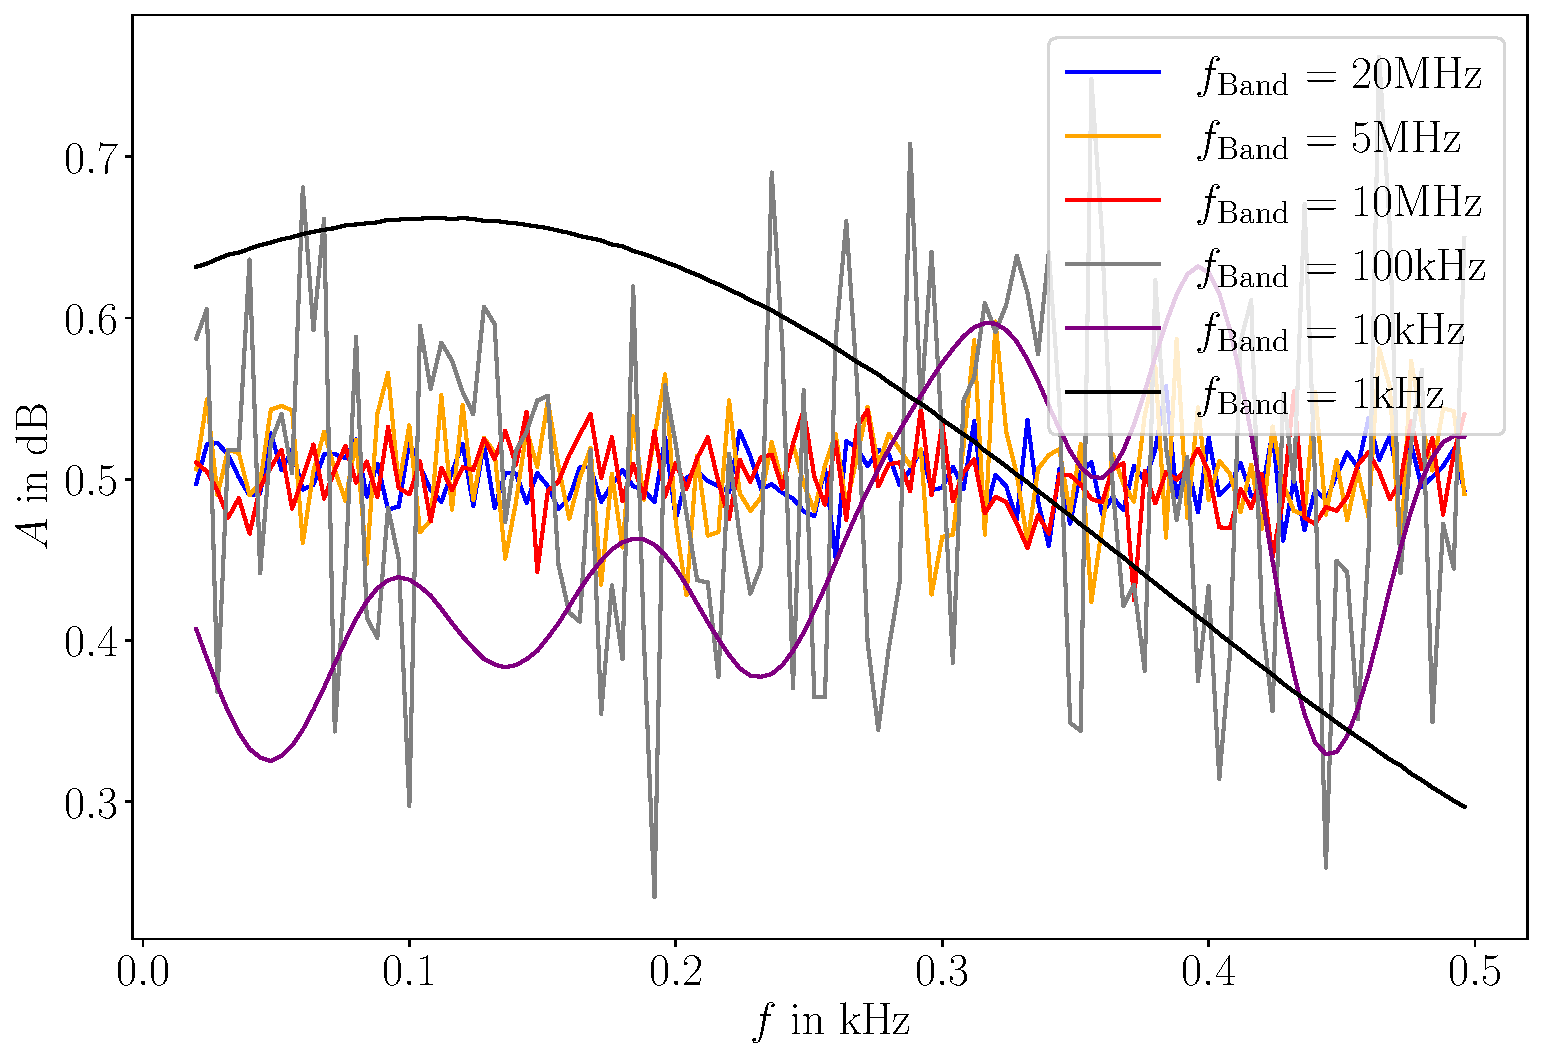
\includegraphics[scale = 0.5]{Manuel/41/Bandbreite.pdf}
    \captionof{figure}{Einfluss Bandbreite im Ausschnitt vom obere Umkehrpunkt der Rechteckschwingung}
    \label{image:bandbreiteRecht}
\end{center} 

